\section{Cross-Embodiment Tactile Unification}
\label{sec:retarget_data}

\subsection{Canonical Surface and Data Contract}
\label{sec:data_contract}
To unify heterogeneous robot morphologies without discarding spatial contact topology, we project all tactile streams onto the official $128\times 128$ MANO UV atlas \citep{romero2017embodied} per hand and horizontally concatenate bimanual recordings into standardized $128\times 256$ streams at 30~FPS.

To guarantee physical rigor and prevent silent evaluation artifacts, every source adheres to a three-part \textbf{data contract}:
\begin{enumerate}[leftmargin=*,nosep]
    \item \textbf{Contact Proxy vs.\ Physical Force:} Uncalibrated UV intensities encode sensor-specific contact proxies---such as fingertip deformation luminance (Sharpa) or elastomer depth proxies (TacVerse)---rather than calibrated Newton forces. Unified UV geometry does not imply unified force semantics across heterogeneous sensors; physical units (N or N$\cdot$m) are reported exclusively when independent external wrench labels pass unit, coordinate-frame, and temporal alignment verification.
    \item \textbf{Observed-Zero vs.\ Unknown:} Each texel separates its contact value from an explicit observation validity indicator, distinguishing the \emph{MANO UV foreground mask} (hand surface vs.\ background) from the \emph{sensor observation mask} (instrumented pads vs.\ uninstrumented fingers or palm). Unobserved regions---which also render dark in UV maps---are excluded from statistics rather than conflated with zero contact.
    \item \textbf{Fixed Global Scaling:} Source streams remain read-only and are mapped through fixed global or training-frozen scalers. Per-frame auto-normalization is strictly prohibited so that relative contact-load trends remain comparable across time.
\end{enumerate}

\subsection{Dual-Route Retargeting}
\label{sec:retarget_pipelines}
Because articulated dexterous hands and two-finger parallel grippers differ in kinematics and sensor mounting, we formulate both pipelines under the same four-stage abstraction---(1)~\emph{Input \& Preprocessing}, (2)~\emph{MANO Alignment}, (3)~\emph{Surface Projection}, and (4)~\emph{Fixed-Scale UV Export}---specializing only the embodiment-dependent alignment and projection steps (Figure~\ref{fig:retarget_pipeline}; implementation constants in Appendix~\ref{app:retarget}).

\begin{figure*}[t]
    \centering
    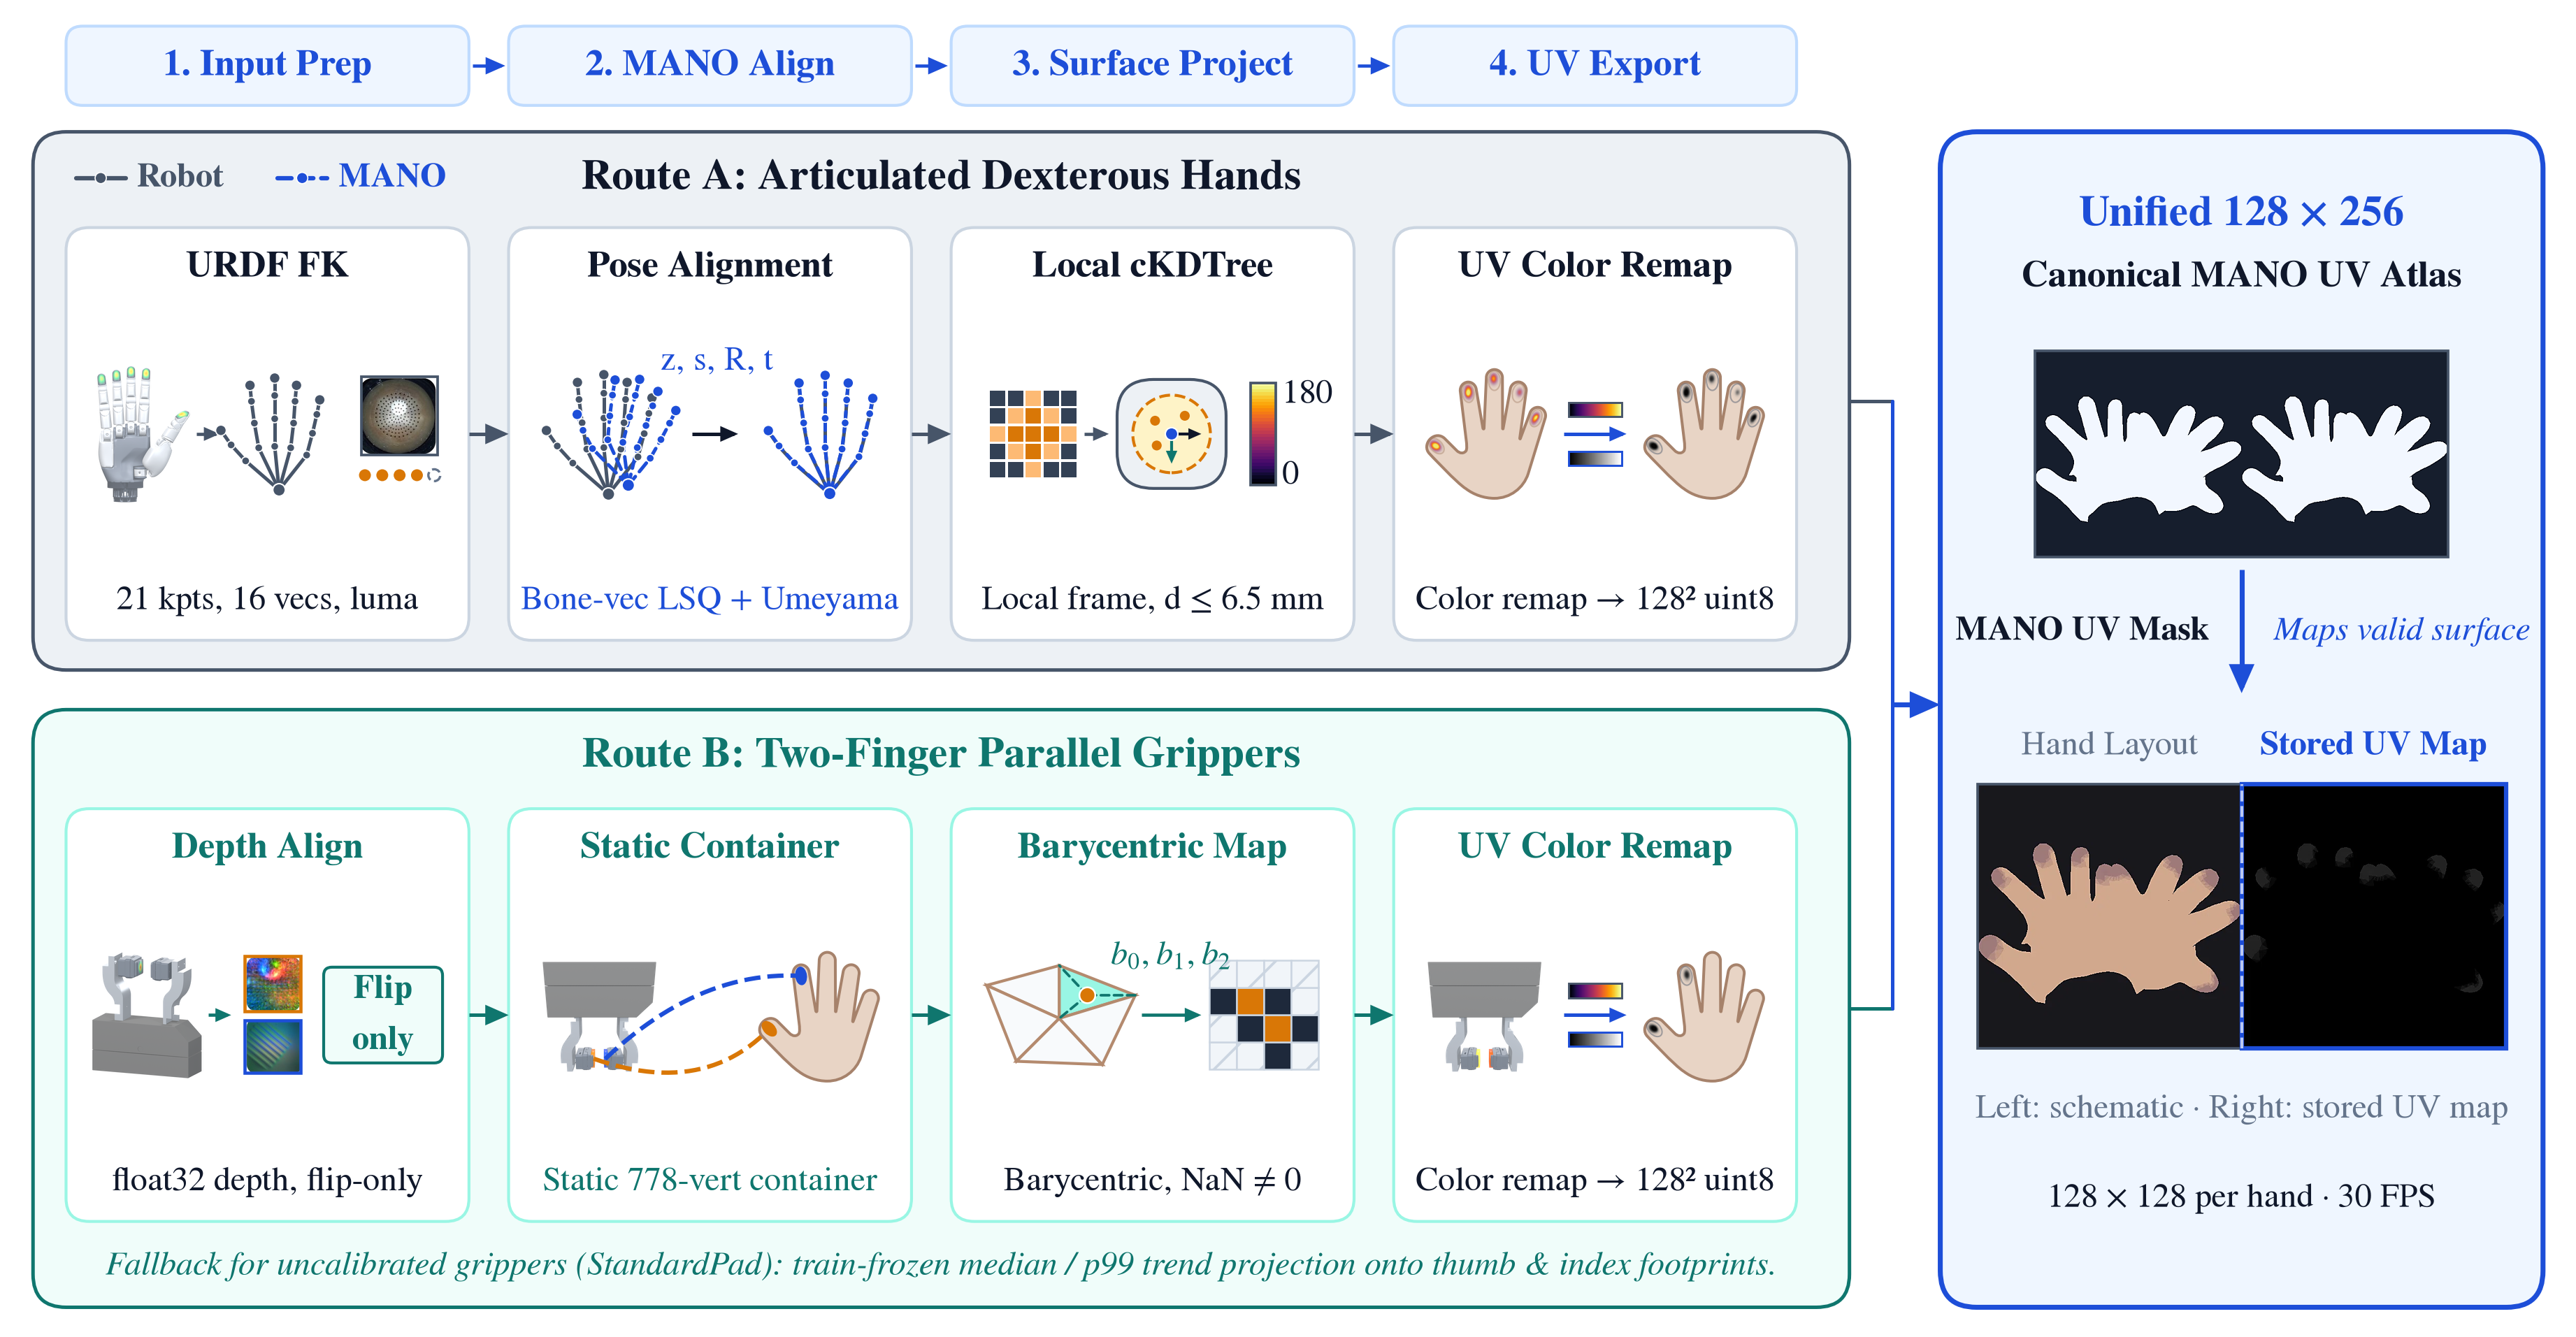
\includegraphics[width=0.95\textwidth]{img/fig2_retarget_pipeline_v2.png}
    \caption{Dual-route cross-embodiment retargeting under a unified four-stage structure. Both routes share the same macro-stages---(1)~Input \& Prep, (2)~MANO Alignment, (3)~Surface Projection, and (4)~Fixed-Scale UV Export---while adapting to embodiment geometry. \textbf{Route~A} maps 22-DoF Sharpa dexterous hands via URDF FK and luminance preprocessing, dynamic warm-started inverse bone-vector fitting with 11-anchor Umeyama seating, distal-phalanx local-frame cKDTree projection, and official UV rasterization with lookup-table recovery. \textbf{Route~B} maps parallel grippers via depth verification and flip-only alignment, static thumb/index pad assignment on a fixed 778-vertex MANO container, barycentric-to-UV texel averaging with \texttt{NaN}-preserving merge, and fixed-range proxy encoding with explicit validity masking (with \texttt{StandardPad} as a fallback for uncalibrated gripper corpora). Both routes converge into unified $128\times 256$ bimanual UV streams under our three-part data contract.}
    \label{fig:retarget_pipeline}
\end{figure*}

\paragraph{Route A: Articulated Dexterous Hands.}
For 22-DoF Sharpa dexterous hands equipped with fingertip deformation arrays, we perform dynamic per-frame kinematic retargeting (without neural training) followed by local-frame tactile projection:
\begin{enumerate}[leftmargin=*,nosep]
    \item \textbf{Input \& Prep (URDF FK \& Tactile Luma):} Because Sharpa's 22 joint angles and MANO's 45-DoF axis-angle rotations differ in joint count, axes, and link lengths, we evaluate the robot URDF via Pinocchio (writing joint states by joint name) to extract 21 MediaPipe-ordered, wrist-centered 3D keypoints $P^{\text{Sharpa}} \in \mathbb{R}^{21 \times 3}$ and 16 unit bone-direction targets $\{\hat{u}^{\text{Sharpa}}_k\}_{k=1}^{16}$. In parallel, observed fingertip tactile streams are converted to luminance and area-downsampled to $240\times 240$; missing finger channels are skipped without fabrication.
    \item \textbf{MANO Alignment (Dynamic Pose Fit \& Umeyama):} We optimize MANO global axis-angle rotation $r \in \mathbb{R}^3$ and 15-DoF PCA latent pose $z \in \mathbb{R}^{15}$ (using a flat-hand mean and $X$-axis mirroring for left hands) via regularized nonlinear least squares:
    \begin{equation}
        \min_{r, z} \sum_{k=1}^{16} \| \hat{u}^{\text{MANO}}_k(r, z) - \hat{u}^{\text{Sharpa}}_k(q) \|_2^2 + \lambda \|z\|_2^2,
    \end{equation}
    where $\lambda = 0.08^2$ and each frame is warm-started from the preceding solution $x_{t-1}$. Matching unit bone directions avoids bone-length mismatch artifacts. A closed-form Umeyama similarity transform $(s, R, t)$ \citep{umeyama1991least} fitted on 11 anchor keypoints (wrist, 5 finger roots, and 5 fingertips) then seats all 778 MANO vertices and 16 joints onto $P^{\text{Sharpa}}$.
    \item \textbf{Surface Projection (Distal-Frame cKDTree):} For each observed finger, we construct a finger-local orthonormal frame anchored at the distal fingertip and scaled by distal bone length, reducing sensitivity to global hand motion. MANO distal vertices (skinning weight $>0.2$) are queried against the manufacturer's $240\times 240\times 3$ sensor point cloud via a KD-tree ($j^* = \arg\min_j \|v^{\text{MANO}}_i - p^{\text{sensor}}_j\|_2$). Only vertices within a $6.5$~mm radius receive luminance values (closer fingers take precedence on overlap), scaled under a fixed saturation map $c = \mathrm{clip}(v/180, 0, 1)$.
    \item \textbf{Fixed-Scale UV Export (Official UV \& LUT):} Vertex intensities are averaged per triangular face (with reversed face winding for left hands) and rasterized onto the official $1024\times 1024$ MANO UV atlas using a cached, pose-invariant face-ID map with 1-pixel seam dilation. The atlas is nearest-neighbor downsampled to $128\times 128$ and inverted through a fixed lookup table back to canonical \texttt{uint8} contact-proxy maps alongside pose metadata and solver diagnostics.
\end{enumerate}

\paragraph{Route B: Two-Finger Parallel Grippers.}
Unlike articulated hands, two-finger parallel grippers lack human-like finger DoFs. Following the same four-stage structure, Route~B replaces dynamic pose fitting and 3D nearest-neighbor search with a static MANO container and direct barycentric texel projection:
\begin{enumerate}[leftmargin=*,nosep]
    \item \textbf{Input \& Prep (Depth Verification \& Flip Align):} Per-pad \texttt{float32} depth maps (reconstructed upstream from visuo-tactile RGB streams using temporally stable maximum-aperture no-contact reference windows) are verified against calibrated reference channels and optionally aligned via flip-only orientation transforms (\texttt{flip\_x}, \texttt{flip\_y}, or \texttt{rotate180}, without rescaling) when reusing left-hand calibrations.
    \item \textbf{MANO Alignment (Static 778-Vertex Container):} Rather than fitting per-frame hand poses, we treat the canonical 778-vertex MANO mesh as a \emph{fixed tactile container}, assigning the left gripper pad to the MANO thumb pad and the right pad to the MANO index pad while leaving the middle, ring, little fingers, and palm explicitly unobserved. Offline geometric calibration stores each valid sensor pixel's MANO face ID and barycentric weights $(b_0, b_1, b_2)$ ($\sum_i b_i = 1$) in a verified lookup table (\texttt{fixed\_mapping.h5}, $<1$~mm surface fit and $<10^{-8}$ vertex-reconstruction check).
    \item \textbf{Surface Projection (Barycentric UV \& \texttt{NaN} Merge):} Because each 3D mesh face shares identical barycentric weights with its 2D UV triangle ($P_{\text{UV}} = \sum_{i=0}^2 b_i\,\mathrm{UV}_i$), valid pixels are pre-mapped directly to $128\times 128$ official UV texel indices with zero per-frame 3D recomputation. Colliding finite depth samples within each finger are averaged per UV texel, and thumb and index rasters are merged with equal weight while preserving every unobserved texel strictly as \texttt{NaN} rather than zero-filling.
    \item \textbf{Fixed-Scale UV Export (Fixed Encode \& Valid Mask):} Finite texels are encoded as \texttt{uint8} contact proxies under a fixed global depth range $c = \mathrm{round}(255\cdot\mathrm{clip}((d - 0.001)/(0.4 - 0.001), 0, 1))$ (with optional \texttt{uint16} depth export over $[-0.001, 0.4]$, reserving $0$ for unknown), paired with an explicit binary observation validity mask (\texttt{valid.png}) separating observed-zero pads from uninstrumented regions.
\end{enumerate}

\paragraph{Extension to Uncalibrated Grippers (\texttt{StandardPad}).}
For parallel-gripper corpora lacking offline pixel-to-mesh geometric calibration, \bench{} provides a fallback \texttt{StandardPad} mode that projects rectangular taxel, depth, or pressure matrices onto the canonical thumb and index UV footprints using training-frozen per-texel median baselines and 99th-percentile scales (zero-centered for signed shear). This preserves spatial and temporal trend structure---onset, load evolution, contact migration, and inter-pad correlation---without assuming metric surface correspondence.

\subsection{Unified Six-Source Corpus and Audit}
\label{sec:dataset_stats}
Table~\ref{tab:dataset_stats} and Figure~\ref{fig:dataset_uv_examples} summarize the six manipulation corpora unified under \bench{}.
Five sources originate from Sharpa dexterous hands (deformation intensity proxies), including \texttt{FTP-1} with partial 3-finger coverage, while \texttt{TacVerse} contributes visuo-tactile parallel-gripper recordings (depth proxies) with explicit observation validity masks.
All unified streams undergo automated contract auditing for schema compliance, frame alignment, and validity-mask integrity, alongside per-frame solver diagnostics (Appendix~\ref{app:audit}).

\begin{figure*}[t]
    \centering
    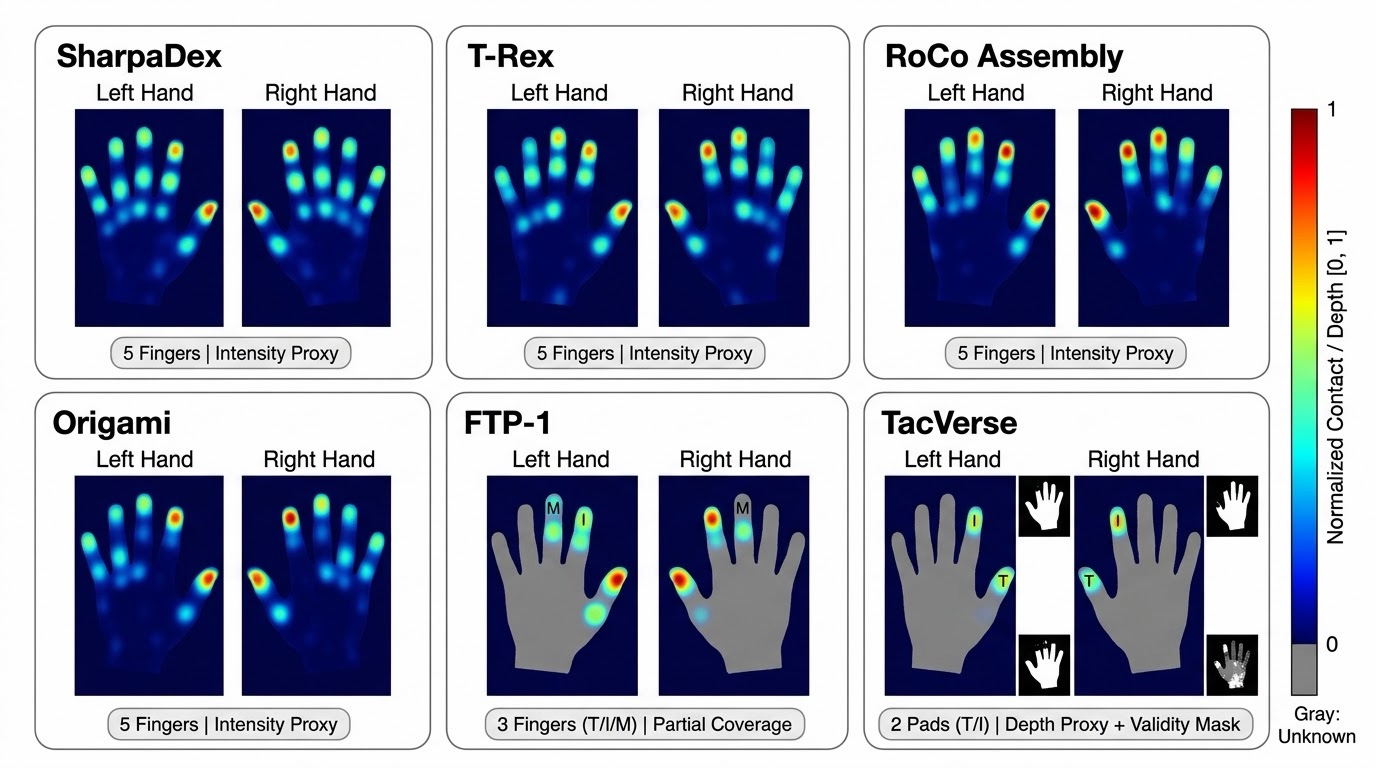
\includegraphics[width=0.95\textwidth]{img/fig3_dataset_uv_examples.jpg}
    \caption{Representative bimanual MANO UV examples across the six unified corpora. Five dexterous-hand sources (\texttt{SharpaDex}, \texttt{T-Rex}, \texttt{RoCo Assembly}, \texttt{Origami}, and partial 3-finger \texttt{FTP-1}) provide contact intensity proxies, while \texttt{TacVerse} provides parallel-gripper depth proxies with explicit validity masks separating observed-zero from unknown texels.}
    \label{fig:dataset_uv_examples}
\end{figure*}

\begin{table*}[t]
\centering
\small
\setlength{\tabcolsep}{5pt}
\begin{tabular}{llccccc}
\toprule
\textbf{Source Corpus} & \textbf{Embodiment} & \textbf{Signal Type} & \textbf{Coverage} & \textbf{Valid Mask} & \textbf{\# Episodes} & \textbf{\# Frames} \\
\midrule
SharpaDex & Dexterous Hand & Intensity proxy & 5 fingers & Planned & \tbd & \tbd \\
T-Rex & Dexterous Hand & Intensity proxy & 5 fingers & Planned & \tbd & \tbd \\
RoCo Assembly & Dexterous Hand & Intensity proxy & 5 fingers & Planned & \tbd & \tbd \\
Origami & Dexterous Hand & Intensity proxy & 5 fingers & Planned & \tbd & \tbd \\
FTP-1 & Dexterous Hand & Intensity proxy & 3 fingers (T/I/M) & Planned & \tbd & \tbd \\
TacVerse & Parallel Gripper & Depth proxy & 2 pads (T/I) & \checkmark & \tbd & \tbd \\
\midrule
\textbf{Total (Unified)} & \textbf{Dexterous + Gripper} & \textbf{2 Proxy Types} & \textbf{2--5 Fingers} & \textbf{Partial} & \tbd & \tbd \\
\bottomrule
\end{tabular}
\caption{Summary of the six tactile corpora unified into the canonical $128\times 256$ (30~FPS) MANO UV format. Raw corpus identifiers and audit details are listed in Appendix~\ref{app:audit}; exact episode and frame counts will be populated upon completion of the six-source manifest.}
\label{tab:dataset_stats}
\end{table*}
